% questions.tex —— 2010 年·普通高等学校招生考试·重庆卷·理科 · 题目内容片段（无答案）
% 由 tools/generate_projects.py 依来源总账自 2010/2010_数学真题_重庆理_试题.md 生成，勿手改（改源 MD 后重跑）
状态：needs-review；依固定候选 PDF 两页（印刷页 577–578）逐题核验，三幅图已矢量重绘。原页未印分值，不补。
\gkpart{一、选择题}
\begin{question}
\gkti{1}在等比数列 $\{a_n\}$ 中，$a_{2010}=8a_{2007}$，则公比 $q$ 的值为（　）

（A）$2$

（B）$3$

（C）$4$

（D）$8$

\end{question}
\begin{question}
\gkti{2}已知向量 $\boldsymbol a$，$\boldsymbol b$ 满足 $\boldsymbol a\cdot\boldsymbol b=0$，$|\boldsymbol a|=1$，$|\boldsymbol b|=2$，则 $|2\boldsymbol a-\boldsymbol b|=$（　）

（A）$0$

（B）$2\sqrt2$

（C）$4$

（D）$8$

\end{question}
\begin{question}
\gkti{3}$\lim\limits_{x\to2}\left(\dfrac{4}{x^2-4}-\dfrac{1}{x-2}\right)=$（　）

（A）$-1$

（B）$-\dfrac14$

（C）$\dfrac14$

（D）$1$

\end{question}
\begin{question}
\gkti{4}设变量 $x$，$y$ 满足约束条件
\nopagebreak[4]
\[\begin{cases}y\geqslant0,\\x-y+1\geqslant0,\\x+y-3\leqslant0,\end{cases}\]
则 $z=2x+y$ 的最大值为（　）

（A）$-2$

（B）$4$

（C）$6$

（D）$8$

\end{question}
\begin{question}
\gkti{5}函数 $f(x)=\dfrac{4^x+1}{2^x}$ 的图象（　）

（A）关于原点对称

（B）关于直线 $y=x$ 对称

（C）关于 $x$ 轴对称

（D）关于 $y$ 轴对称

\Needspace{0.4\textheight}
\end{question}
\begingroup
\renewenvironment{question}{\Needspace{0.5\textheight}}{}
\begin{question}
\gkti{6}已知函数 $y=\sin(\omega x+\varphi)$（$\omega>0$，$|\varphi|<\dfrac{\pi}{2}$）的部分图象如图所示，则（　）

（A）$\omega=1$，$\varphi=\dfrac{\pi}{6}$

（B）$\omega=1$，$\varphi=-\dfrac{\pi}{6}$

（C）$\omega=2$，$\varphi=\dfrac{\pi}{6}$

（D）$\omega=2$，$\varphi=-\dfrac{\pi}{6}$
\nopagebreak[4]
\begin{center}% 2010 年重庆卷理科第 6 题：y=sin(ωx+φ) 的部分图象。
% 来源 PDF：普通高考/2010/2010重庆理.pdf，SHA-256 e981a8805207e307d0ec0d8ef50ac0e0cbf93eec9559a29fb88591b483ae0136。
% 原页：第 1 页（A3 三栏）第 1 栏中部，书页码 577。
% 重绘依据（按原页矢量路径换算，横纵同为每单位 24 pt）：
%   曲线自 y 轴上的点 (0,-1/2) 起画，在 x=π/3 处取最大值 1，在 x=7π/12 处与 x 轴相交，
%   一直画到 x=π（恰一个周期，右端回到 y=-1/2）；峰值处画虚线：水平段连到 y 轴、竖段落到 x 轴；
%   x 轴左端伸到 x=-1，y 轴上下均伸出 x 轴。
\begin{tikzpicture}[scale=0.8, semithick]
  % 坐标轴
  \draw[->] (-1.35,0) -- (4.15,0) node[below] {$x$};
  \draw[->] (0,-1.6) -- (0,1.55) node[left] {$y$};
  % 曲线 y=sin(2x-π/6)，x∈[0,π]
  \draw[thick] plot[domain=0:3.14159265, samples=160]
    (\x, {sin(2*\x r - pi/6 r)});
  % 峰值的虚线标注
  \draw[dashed] (0,1) -- ({pi/3},1);
  \draw[dashed] ({pi/3},1) -- ({pi/3},0);
  % 刻度与文字
  \node[left] at (-0.06,1) {$1$};
  \node[below left] at (0,0) {$O$};
  \node[below] at ({pi/3},-0.12) {$\dfrac{\pi}{3}$};
  \node[below] at ({7*pi/12},-0.12) {$\dfrac{7\pi}{12}$};
\end{tikzpicture}
\end{center}
\nopagebreak[4]
\end{question}
\endgroup
\begin{question}
\gkti{7}已知 $x>0$，$y>0$，$x+2y+2xy=8$，则 $x+2y$ 的最小值是（　）

（A）$3$

（B）$4$

（C）$\dfrac92$

（D）$\dfrac{11}{2}$

\end{question}
\begin{question}
\gkti{8}直线 $y=\dfrac{\sqrt3}{3}x+\sqrt2$ 与圆心为 $D$ 的圆
\nopagebreak[4]
\[\begin{cases}x=\sqrt3+\sqrt3\cos\theta,\\y=1+\sqrt3\sin\theta,\end{cases}\quad(\theta\in[0,2\pi))\]
交于 $A$，$B$ 两点，则直线 $AD$ 与 $BD$ 的倾斜角之和为（　）

（A）$\dfrac76\pi$

（B）$\dfrac54\pi$

（C）$\dfrac43\pi$

（D）$\dfrac53\pi$

\end{question}
\begin{question}
\gkti{9}某单位安排 $7$ 位员工在 $10$ 月 $1$ 日至 $7$ 日值班，每天 $1$ 人，每人值班 $1$ 天，若 $7$ 位员工中的甲、乙排在相邻两天，丙不排在 $10$ 月 $1$ 日，丁不排在 $10$ 月 $7$ 日，则不同的安排方案共有（　）

（A）$504$ 种

（B）$960$ 种

（C）$1008$ 种

（D）$1108$ 种

\end{question}
\begin{question}
\gkti{10}到两互相垂直的异面直线的距离相等的点，在过其中一条直线且平行于另一条直线的平面内的轨迹是（　）

（A）直线

（B）椭圆

（C）抛物线

（D）双曲线

\end{question}
\gkpart{二、填空题}
\begin{question}
\gkti{11}已知复数 $z=1+\mathrm{i}$，则 $\dfrac2z-z=$ $\underline{\qquad}$。

\end{question}
\begin{question}
\gkti{12}设 $U=\{0,1,2,3\}$，$A=\{x\in U\mid x^2+mx=0\}$，若 $\complement_U A=\{1,2\}$，则实数 $m=$ $\underline{\qquad}$。

\end{question}
\begin{question}
\gkti{13}某篮球队员在比赛中每次罚球的命中率相同，且在两次罚球中至多命中一次的概率为 $\dfrac{16}{25}$，则该队员每次罚球的命中率为 $\underline{\qquad}$。

\end{question}
\begin{question}
\gkti{14}已知以 $F$ 为焦点的抛物线 $y^2=4x$ 上的两点 $A$、$B$ 满足 $\overrightarrow{AF}=3\overrightarrow{FB}$，则弦 $AB$ 的中点到准线的距离为 $\underline{\qquad}$。

\end{question}
\begin{question}
\gkti{15}已知函数 $f(x)$ 满足：$f(1)=\dfrac14$，$4f(x)f(y)=f(x+y)+f(x-y)$（$x$，$y\in\mathbf R$），则 $f(2010)=$ $\underline{\qquad}$。

\end{question}
\gkpart{三、解答题}
\begin{question}
\gkti{16}设函数 $f(x)=\cos\left(x+\dfrac23\pi\right)+2\cos^2\dfrac x2$，$x\in\mathbf R$。

（1）求 $f(x)$ 的值域；

（2）记 $\triangle ABC$ 的内角 $A$，$B$，$C$ 的对边长分别为 $a$，$b$，$c$，若 $f(B)=1$，$b=1$，$c=\sqrt3$，求 $a$ 的值。

\end{question}
\begin{question}
\gkti{17}在甲、乙等 $6$ 个单位参加的一次“唱读讲传”演出活动中，每个单位的节目集中安排在一起，若采用抽签的方式随机确定各单位的演出顺序（序号为 $1$，$2$，$\cdots$，$6$），求：

（1）甲、乙两单位的演出序号至少有一个为奇数的概率；

（2）甲、乙两单位之间的演出单位个数 $\xi$ 的分布列与期望。

\end{question}
\begin{question}
\gkti{18}已知函数 $f(x)=\dfrac{x-1}{x+a}+\ln(x+1)$，其中实数 $a\neq1$。

（1）若 $a=2$，求曲线 $y=f(x)$ 在点 $(0,f(0))$ 处的切线方程；

（2）若 $f(x)$ 在 $x=1$ 处取得极值，试讨论 $f(x)$ 的单调性。

\Needspace{0.4\textheight}
\end{question}
\begingroup
\renewenvironment{question}{\Needspace{0.5\textheight}}{}
\begin{question}
\gkti{19}如图，四棱锥 $P-ABCD$ 中，底面 $ABCD$ 为矩形，$PA\perp$ 底面 $ABCD$，$PA=AB=\sqrt6$，点 $E$ 是棱 $PB$ 的中点。

（1）求直线 $AD$ 与平面 $PBC$ 的距离；

（2）若 $AD=\sqrt3$，求二面角 $A-EC-D$ 的平面角的余弦值。
\nopagebreak[4]
\begin{center}% 2010 年重庆卷理科第 19 题：四棱锥 P-ABCD，底面 ABCD 为矩形，PA⊥底面，E 为棱 PB 的中点。
% 来源 PDF：普通高考/2010/2010重庆理.pdf，SHA-256 e981a8805207e307d0ec0d8ef50ac0e0cbf93eec9559a29fb88591b483ae0136。
% 原页：第 2 页（A3 三栏）第 1 栏上部，书页码 578。
% 重绘依据：按原页矢量路径逐段提取顶点位置（以 BC=4 为单位长）：
%   B(0,0)、C(4,0)、A(2,2)、D(6,2)、P(2,7.66)、E(1,3.83)，P 在 A 的正上方、E 为 PB 中点。
% 实线：BC、CD、CE、PB、PC、PD；虚线：PA、AB、AD、AC、AE、DE（与原页虚线段一一对应）。
% 原页在顶点 A 处画一个小叉表示该顶点被遮挡，此图照录。
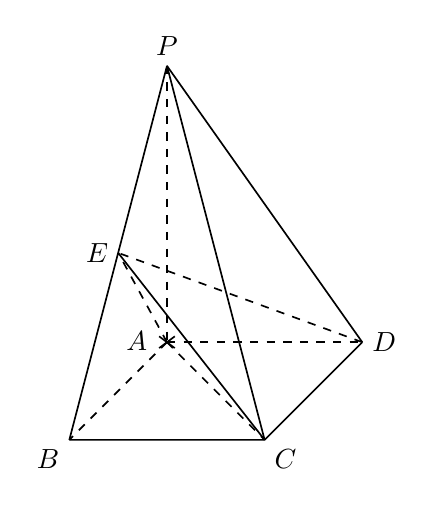
\begin{tikzpicture}[scale=0.62, semithick]
  \coordinate (B) at (0,0);
  \coordinate (C) at (4,0);
  \coordinate (A) at (2,2);
  \coordinate (D) at (6,2);
  \coordinate (P) at (2,7.66);
  \coordinate (E) at (1,3.83);

  % 可见棱
  \draw (B) -- (C) -- (D);
  \draw (P) -- (B);
  \draw (P) -- (C);
  \draw (P) -- (D);
  \draw (C) -- (E);

  % 被遮挡的棱
  \draw[dashed] (P) -- (A);
  \draw[dashed] (A) -- (B);
  \draw[dashed] (A) -- (D);
  \draw[dashed] (A) -- (C);
  \draw[dashed] (A) -- (E);
  \draw[dashed] (D) -- (E);

  % 原页在 A 处的遮挡叉号
  \draw[line width=0.6pt] (1.84,1.88) -- (2.16,2.12);
  \draw[line width=0.6pt] (1.84,2.12) -- (2.16,1.88);

  \node[above]       at (P) {$P$};
  \node[left]        at (E) {$E$};
  \node at (1.38,2.02) {$A$};
  \node[below left]  at (B) {$B$};
  \node[below right] at (C) {$C$};
  \node[right]       at (D) {$D$};
\end{tikzpicture}
\end{center}
\nopagebreak[4]
\Needspace{0.4\textheight}
\end{question}
\endgroup
\begingroup
\renewenvironment{question}{\Needspace{0.5\textheight}}{}
\begin{question}
\gkti{20}已知以原点 $O$ 为中心，$F(\sqrt5,0)$ 为右焦点的双曲线 $C$ 的离心率 $e=\dfrac{\sqrt5}{2}$。

（1）求双曲线 $C$ 的标准方程及其渐近线方程；

（2）如图，已知过点 $M(x_1,y_1)$ 的直线 $l_1$：$x_1x+4y_1y=4$ 与过点 $N(x_2,y_2)$（其中 $x_2\neq x_1$）的直线 $l_2$：$x_2x+4y_2y=4$ 的交点 $E$ 在双曲线 $C$ 上，直线 $MN$ 与两条渐近线分别交于 $G$、$H$ 两点，求 $\triangle OGH$ 的面积。
\nopagebreak[4]
\begin{center}% 2010 年重庆卷理科第 20 题：双曲线 C（中心 O，右焦点 F）与两条渐近线、直线 l1、l2、MN 的位置图。
% 来源 PDF：普通高考/2010/2010重庆理.pdf，SHA-256 e981a8805207e307d0ec0d8ef50ac0e0cbf93eec9559a29fb88591b483ae0136。
% 原页：第 2 页（A3 三栏）第 2 栏中部，书页码 578。
% 重绘依据：按原页矢量路径换算成以 a=2 为单位的坐标（每单位 14.4 pt）：
%   原点 O(0,0)；x 轴 -1.97～6.64，y 轴 -3.93～3.69；
%   双曲线只画右支 x=2√(1+y²)（原页即只画右支，线较粗）；
%   两条渐近线均自 O 向右上方、右下方画出（原页也不画左半段）；
%   l1 过 M(-0.64,-0.98)，l2 过 N(1.69,0.42)，二者交于 E(5.3,-2.46)（在右支上）；
%   MN 过 M、N，与 y=x/2 交于 G(5.96,2.99)、与 y=-x/2 交于 H(0.54,-0.27)；
%   M、N 在原页为实心圆点，E、G、H 无圆点。
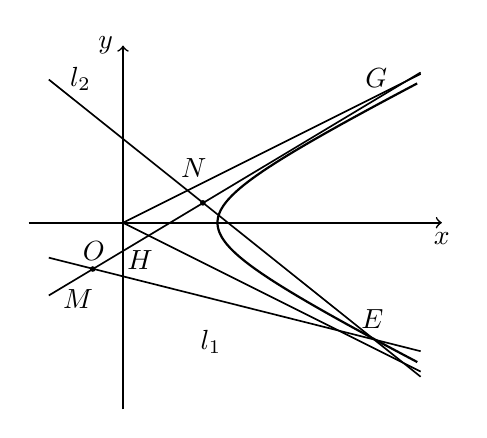
\begin{tikzpicture}[scale=0.6, semithick]
  \coordinate (O) at (0,0);
  \coordinate (M) at (-0.64,-0.98);
  \coordinate (N) at (1.69,0.42);
  \coordinate (E) at (5.30,-2.46);
  \coordinate (G) at (5.96,2.99);
  \coordinate (H) at (0.54,-0.27);

  % 坐标轴
  \draw[->] (-2.0,0) -- (6.75,0) node[below] {$x$};
  \draw[->] (0,-3.95) -- (0,3.75) node[left] {$y$};

  % 双曲线右支 x^2/4-y^2=1
  \draw[thick] plot[domain=-2.95:2.95, samples=140, variable=\y]
    ({2*sqrt(1+\y*\y)}, \y);

  % 渐近线 y=±x/2（只画右半）
  \draw (O) -- (6.30,3.15);
  \draw (O) -- (6.30,-3.15);

  % l1（过 M）、l2（过 N）、MN
  \draw (-1.57,-0.74) -- (6.30,-2.72);
  \draw (-1.57,3.03) -- (6.30,-3.26);
  \draw (-1.57,-1.54) -- (6.30,3.18);

  % 点 M、N 处实心圆点
  \fill (M) circle (1.7pt);
  \fill (N) circle (1.7pt);

  % 文字（位置照原页）
  \node at (-0.90,3.05) {$l_2$};
  \node at (1.86,-2.52) {$l_1$};
  \node at (-0.62,-0.60) {$O$};
  \node at (-0.95,-1.62) {$M$};
  \node at (1.50,1.16) {$N$};
  \node at (5.28,-2.03) {$E$};
  \node at (5.36,3.06) {$G$};
  \node at (0.36,-0.80) {$H$};
\end{tikzpicture}
\end{center}
\nopagebreak[4]
\end{question}
\endgroup
\begin{question}
\gkti{21}在数列 $\{a_n\}$ 中，$a_1=1$，$a_{n+1}=ca_n+c^{n+1}(2n+1)$（$n\in\mathbf N^*$），其中实数 $c\neq0$。

（1）求 $\{a_n\}$ 的通项公式；

（2）若对一切 $k\in\mathbf N^*$ 有 $a_{2k}>a_{2k-1}$，求 $c$ 的取值范围。

\end{question}